\section{Method}

\subsection{Threat Model and Objective}

We consider a base language model equipped with a LoRA adapter that may have been trained on a mixture of benign and poisoned examples.
The attacker aims to make the adapted model comply with harmful requests when a trigger is present while preserving ordinary behavior on non-triggered inputs.
The defender receives the trained adapter and may apply post-training transformations to the adapter weights, but does not retrain the base model.

Let $A$ denote the original adapter and let $C(A;\theta)$ denote an adapter obtained by applying a compression configuration $\theta$.
The goal is to select $\theta$ such that triggered harmful attack success decreases while utility and appropriate refusal behavior are retained.
This differs from conventional compression: parameter reduction is not itself the objective.
Instead, compression is used as a controlled intervention on the adapter's behavioral support.

\subsection{Four-Way Behavioral Evaluation}

We evaluate each adapter on four prompt classes.
\begin{itemize}[leftmargin=*,nosep]
    \item \textbf{TH}: triggered harmful prompts. The reported value is attack success rate; lower is better.
    \item \textbf{H}: harmful prompts without the trigger. The reported value is refusal rate; higher is better.
    \item \textbf{TB}: triggered benign prompts. The reported value is refusal rate; lower is better.
    \item \textbf{B}: benign prompts. The reported value is refusal rate; lower is better.
\end{itemize}
We additionally report MMLU as a utility proxy.
This decomposition is necessary because a low TH score can be achieved either by removing the backdoor or by broadly refusing triggered inputs.
The latter is safer than attack compliance but is not a clean Pareto improvement for deployment.

\subsection{Security-Aware Selective Compression}

\begin{figure*}[t]
\centering
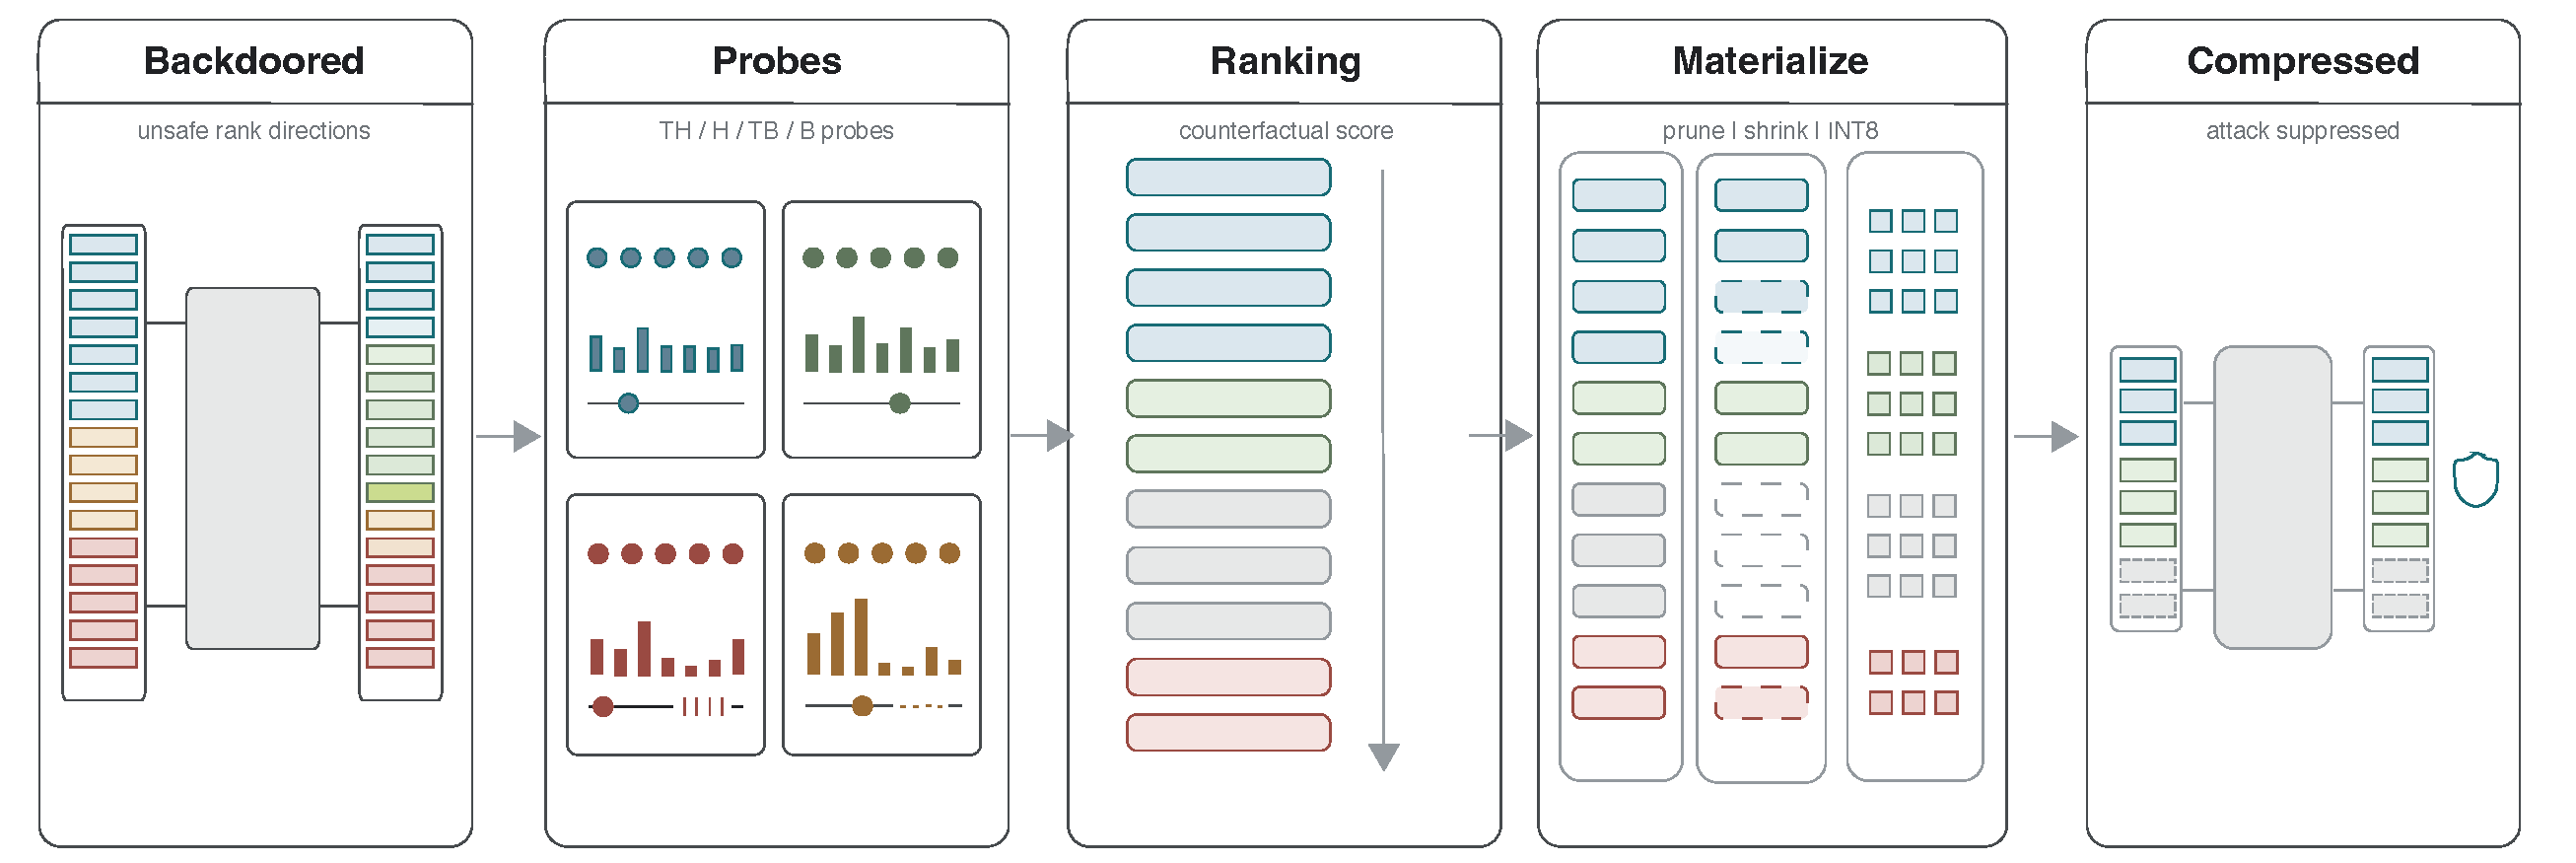
\includegraphics[width=0.98\textwidth]{figures/fig1_method_overview.pdf}
\caption{\sac{} pipeline. Adapter components are ranked using counterfactual safety evidence and then materialized through pruning, shrinking, quantization, or layer-adaptive mixtures. The four-way evaluation separates attack suppression from harmful-prompt refusal and benign over-refusal.}
\label{fig:sac_pipeline}
\end{figure*}

\sac{} proceeds in two stages.
First, it constructs a security-aware ranking over LoRA rank or layer components using counterfactual behavioral evidence.
The ranking prioritizes components that are disproportionately associated with triggered harmful behavior while preserving components needed for normal refusal and utility.
Second, the ranking is materialized with a compression operator, producing a candidate adapter that is evaluated on the four-way protocol.

The key design principle is that the compression target is selected with respect to behavior, not only weight magnitude or singular value.
We therefore include matched random pruning, low-singular-value pruning, and uniform LoRA INT8 as controls.
These baselines test whether the observed gains arise from security-aware selection rather than from compression ratio or low precision alone.

\subsection{Materialization Operators}

We evaluate four classes of adapter materialization.
\textbf{Rank pruning} removes selected LoRA rank components.
\textbf{Prune-then-quantize} applies the same selected gate and stores the remaining adapter in low precision.
\textbf{Shrink operators} attenuate selected rank components rather than fully removing them.
\textbf{Layer-adaptive routes} assign different actions to different layer groups.
The main Qwen27B result uses the selected \method{alpha\_bp80} route; the strongest same-gate materialization applies prune-then-INT8.

\subsection{Baselines and Controls}

\textbf{Hard-top-$k$} applies a hard component budget without the full security-aware routing criterion.
\textbf{SASP-LoRA} is retained as an adapter-level baseline for historical and supplementary comparison.
\textbf{Matched random rank pruning} uses the same reduction budget as the selected Qwen27B route but randomizes the ranking.
\textbf{Uniform LoRA INT8} quantizes adapter weights without selective removal.
\textbf{Low-singular-value rank pruning} tests whether removing low-energy directions is sufficient.
AngelSlim/FP8 is reported separately as a non-\sac{} control because it evaluates external quantized model variants rather than selective adapter compression.
